% BASIC SETTINGS
\documentclass[a4paper,12pt]{article} % Set paper size and document type
\usepackage{lmodern} % Use a slightly nicer looking font
\usepackage{url} % Proper formatting for URLs
\usepackage{graphicx} % Handle inclusion of non-PDF graphics
\usepackage{subfig} % Allow sub-figures inside a figure
\usepackage{enumitem} % Allow lists to pick up numbering where the last list left off

% Change margins - default margins are too broad
\usepackage[margin=20mm]{geometry}

% SOURCE CODE LISTING SETTINGS 
% https://en.wikibooks.org/wiki/LaTeX/Source_Code_Listings
\usepackage{listings}
\usepackage{color}
\usepackage{amssymb}

% Color definitions for source code listings
\definecolor{mygreen}{rgb}{0,0.6,0}
\definecolor{mygray}{rgb}{0.5,0.5,0.5}
\definecolor{mymauve}{rgb}{0.58,0,0.82}

% Formatting (line breaks, spacing, etc...) for code
\lstset{ 
  backgroundcolor=\color{white},   % choose the background color; you must add \usepackage{color} or \usepackage{xcolor}
  basicstyle=\footnotesize,        % the size of the fonts that are used for the code
  breakatwhitespace=false,         % sets if automatic breaks should only happen at whitespace
  breaklines=true,                 % sets automatic line breaking
  captionpos=b,                    % sets the caption-position to bottom
  commentstyle=\color{mygreen},    % comment style
  deletekeywords={...},            % if you want to delete keywords from the given language
  escapeinside={\%*}{*)},          % if you want to add LaTeX within your code
  extendedchars=true,              % lets you use non-ASCII characters; for 8-bits encodings only, does not work with UTF-8
  frame=single,	                   % adds a frame around the code
  keepspaces=true,                 % keeps spaces in text, useful for keeping indentation of code (possibly needs columns=flexible)
  keywordstyle=\color{blue},       % keyword style
  otherkeywords={*,...},           % if you want to add more keywords to the set
  numbers=left,                    % where to put the line-numbers; possible values are (none, left, right)
  numbersep=5pt,                   % how far the line-numbers are from the code
  numberstyle=\tiny\color{mygray}, % the style that is used for the line-numbers
  rulecolor=\color{black},         % if not set, the frame-color may be changed on line-breaks within not-black text (e.g. comments (green here))
  showspaces=false,                % show spaces everywhere adding particular underscores; it overrides 'showstringspaces'
  showstringspaces=false,          % underline spaces within strings only
  showtabs=false,                  % show tabs within strings adding particular underscores
  stepnumber=2,                    % the step between two line-numbers. If it's 1, each line will be numbered
  stringstyle=\color{mymauve},     % string literal style
  tabsize=2,	                   % sets default tabsize to 2 spaces
  title=\lstname                   % show the filename of files included with \lstinputlisting; also try caption instead of title
}

% Set document title and author
\title{ Modelling Uncertainty}
\author{SC03 Group 1 \\\\ Stefanie Tan Hui Zhen 1006073 \\ Abhijith Kizhakke Chittadath 1006276 \\ Ansley Tan An Qing 1006070 \\ Aaron Zhe Yu Tua 1006276 \\ Patrick Phone Myat Mo 1006084 }
\date {}
% Document body
\begin{document}

\maketitle % Insert the title, author, and date


\clearpage
\vspace{10mm}
\section{Question 1} %  Create a section


% Include code from a file with filename indicated
\vspace{5mm}




\centerline {p : probability of going up by 1 unit}
\centerline {1 - p : probability of going down by 1 unit }
\vspace{5mm}
\centerline { p( $X_i$ = 1) = p ,  p( $X_i$ = -1) = q}
\centerline { q = 1 - p }



\centerline {$S_n$ = $\sum_{i=1}^{n} X_i$}

\vspace{2mm}

1(a) 
                         

\centerline {Largest value of $S_n$ : all values of $X_i$ = 1}
\centerline {  $\sum_{i=1}^{n} 1$ = n }
\vspace{5mm}

\centerline {Smallest value of $S_n$ : all values of $X_i$ = - 1}
\centerline {  $\sum_{i=1}^{n} -1$ = -n }



\noindent
1(b) 

\vspace{5mm}

\centerline {P( $S_n$ = 0 ) as a function of n when :}
\centerline {Let Y $\sim$ Binomial ( n,p ) where Y is the no. of days when}
\centerline {$X_i$ is 1}

\vspace{5mm}
\centerline {For $S_n$ = 0, while n is even :}
\centerline {Equal no. of days when $X_i$ = -1}
\centerline {Y = n/2}
\vspace{5mm}
\centerline {While n is odd : Impossible for Sn = 0}
\centerline{ P ( $S_n$ = 0 $\mid$ n is an odd number ) = 0 }
\centerline{ P ( $S_n$ = 0 $\mid$ n is an even number) = $N\choose k$}

\noindent
1(c)

\centerline {P ($S_n$ = 2m + 1) where m is group number ( 1 ) , $S_n$ = 2(1) + 1 = 3}
\centerline {P ($S_n$ = 3 $\mid$ even n ) = 0}
\centerline {For $S_n$ = 3, 3 + ( n -3 )/2 cases of $X_i$ = 1}
\centerline {(n-3)/2 cases of $X_i$ = -1}

\vspace{5mm}

\centerline{ P ( $S_n$ = 3 $\mid$ odd n ) = $n\choose (n-3)/2$  $p^{3+(n-3)/2}$ $p^{(n-3)/2}$ }

\centerline{= $n\choose (n-3)/2$  $p^{3+(n-3)/2}$ $p^{(n-3)/2}$ }

\[ \ P(S_n=3) = \left\{ 
\begin{array}{l l}



\ 0 & if \ n \ is \ odd\\
\  \ {n\choose (n-3)/2 )} \ p^{3+(n-3)/2}\ p^{(n-3)/2}\ & if \ n \ is \ even\\


\end{array} \right\}
\] 


\noindent
1(d)

\centerline {$X_i$ $\sim$ Bernoulli (p)}
\centerline {Let Y $\sim$ binomial (n,p), where Y is the no. of days where $X_i$ = 1}
\centerline {$S_n$ = Y -  (n - Y)  }
\centerline {$S_n$ = 2Y - n}




\noindent
1(e)

\centerline {E[Y] = np}
\centerline {E[$S_n$]  = E[ 2Y - n ] = 2E[Y] - n = 2np - n}
\centerline {E[$S_n$] = (2p - 1)n}

\clearpage
\centerline {Var[$S_n$] = Var[$2Y - n$] = Var[2Y] - Var[n] = 4Var[Y] - Var[n]}
\centerline {Var[n] = 0 , n =/= Random Variable}
\centerline {4Var[Y] - Var[n] = 4Var[Y]}
\centerline {Var[Y] = np(1-p) = npq , Variance of Binomial Distribution}
\centerline {Var[$S_n$] = 4Var[y] = 4npq}

\vspace{5mm}


\noindent
1(f)
\noindent
$S_n$ exists as a binomial distribution as it is only a scalar and stretching translation of a binomial distribution. When n is large, we can deduce that it carries the same mean and variance.

\centerline { $\mu$ = E[$S_n$] = n(2p-1)  ; $\sigma$$^{2}$ = 4npq}
\centerline{ $S_n$ $\sim$ normal( n(2p-1) , 4npq )}


\section{Question 2} 

\centerline {NEEDS UPDATING }
\centerline {P($X_i$ = 1) = p , P($X_j$= -1) = q , where 0 < p < 1}
\centerline {$S_n$ refers to net amount of investment units e.g for step 3, i = 2}
\centerline {hence, max$S_n$ = n}
\centerline {P(max$S_n$) = {$p^{n}$} }
\centerline {min$S_n$ = -n}
\centerline { P(min$S_n$ = $q_n$}
\vspace{5mm}

\noindent
2(a)

\centerline {N = k + $S_n$, where N = 3 and k = 1 (given) => $S_n$ = 2}
\centerline {hence win condition : no. of p = 2 + no. of q}
\vspace{5mm}
\centerline {Probability of winning , P(win) = $p^2 + pqp^2 + pqpqp^2 +...$}
\centerline {= $p^2 + pqp^2 + p^2q^2p^2 + p^3q^3p^2 + ...$}
\centerline{= $p^2(1 + pq + (pq)^2 + (pq)^3 + ... )$}
\centerline {= $p^2$/(1 - pq)}
\centerline {= $p^2$ / ($p^2 - p + 1$ )}
\centerline {= no. of p - no. of q}

\vspace{5mm}

\noindent
2(b)

\centerline{Let B = probability of ($X_i$ = 1) , UPDATING}

\centerline{A = probability of winning with k}

\centerline{Law of probability : P(B) = P( B$\sim$A)P(A) + Updating}

\centerline{Whole question needs updating}

\vspace{5mm}
\noindent
2(c)

\centerline{$P_k$ = $p^(1-Q)$ CONTINUE FROM HERE}



















% Forces content onto the next page, useful for documents which should look nice when printed out
\clearpage

\noindent
We can also place code directly into latex without importing it from a file:

% Include code inline
\vspace{5mm}
\begin{lstlisting}[language=Python]
print("Hi, I'm Python 3!")
\end{lstlisting}
\vspace{5mm}

\subsection{First subsection} % Create a subsection

We can create and format mathematical expressions like so:

\vspace{2mm}
% Format a mathematical expression
$$x' = x \cdot s cos \theta - y \cdot s sin \theta + t_x$$
$$y' = x \cdot s sin \theta + y \cdot s cos \theta + t_y$$
\vspace{2mm}

\noindent
We can also make a nice list:

% Make a list
\vspace{2mm}
\begin{enumerate}
\item I am the first thing in the list
\item I am the second thing in the list
\end{enumerate}
\vspace{2mm}

\noindent
We can inline mathematical expressions such as this one "$4 \sigma_0$" using the "\$" sign. We can make mathematical expressions that occupy their own line, like this: 
\vspace{2mm}
$$u = (x - x_0) \frac{1}{4 \sigma_0} cos \theta_0 - (y - y_0) \frac{1}{4 \sigma_0} sin \theta_0 + 4 = (0 - 16) \frac{1}{4} - 0 + 4$$
\vspace{2mm}

\subsection{Second subsection}

We can also make tables and charts using the array type like so:

% Make an array or table
\vspace{2mm}
\[ \phi = \left\{ 
\begin{array}{l l}

\theta_0 + \theta_{pt} & if \ \theta_0 + \theta_{pt} \in [0,2 \pi)\\ 

\theta_0 + \theta_{pt} + 2 \pi & if \ \theta_0 + \theta_{pt} < 0\\
\theta_0 + \theta_{pt} - 2 \pi & if \ \theta_0 + \theta_{pt} \ge 2 \pi\\

\end{array} \right\}
\] 
\vspace{2mm}

\noindent
I can start an enumerated list of items here...

\vspace{5mm}
\begin{enumerate}
\item One thing
\item Another thing
\end{enumerate}
\vspace{5mm}

\noindent
And then...

\section{Second section}

...I can continue it here!

\vspace{5mm}
\begin{enumerate}[resume]
\item Yet more stuff
\item Some other things
\end{enumerate}
\vspace{5mm}

Inserting figures is also relatively easy to do: 

\vspace{5mm}
% Insert a figure with an image
\begin{figure}[!ht]
  \centering
  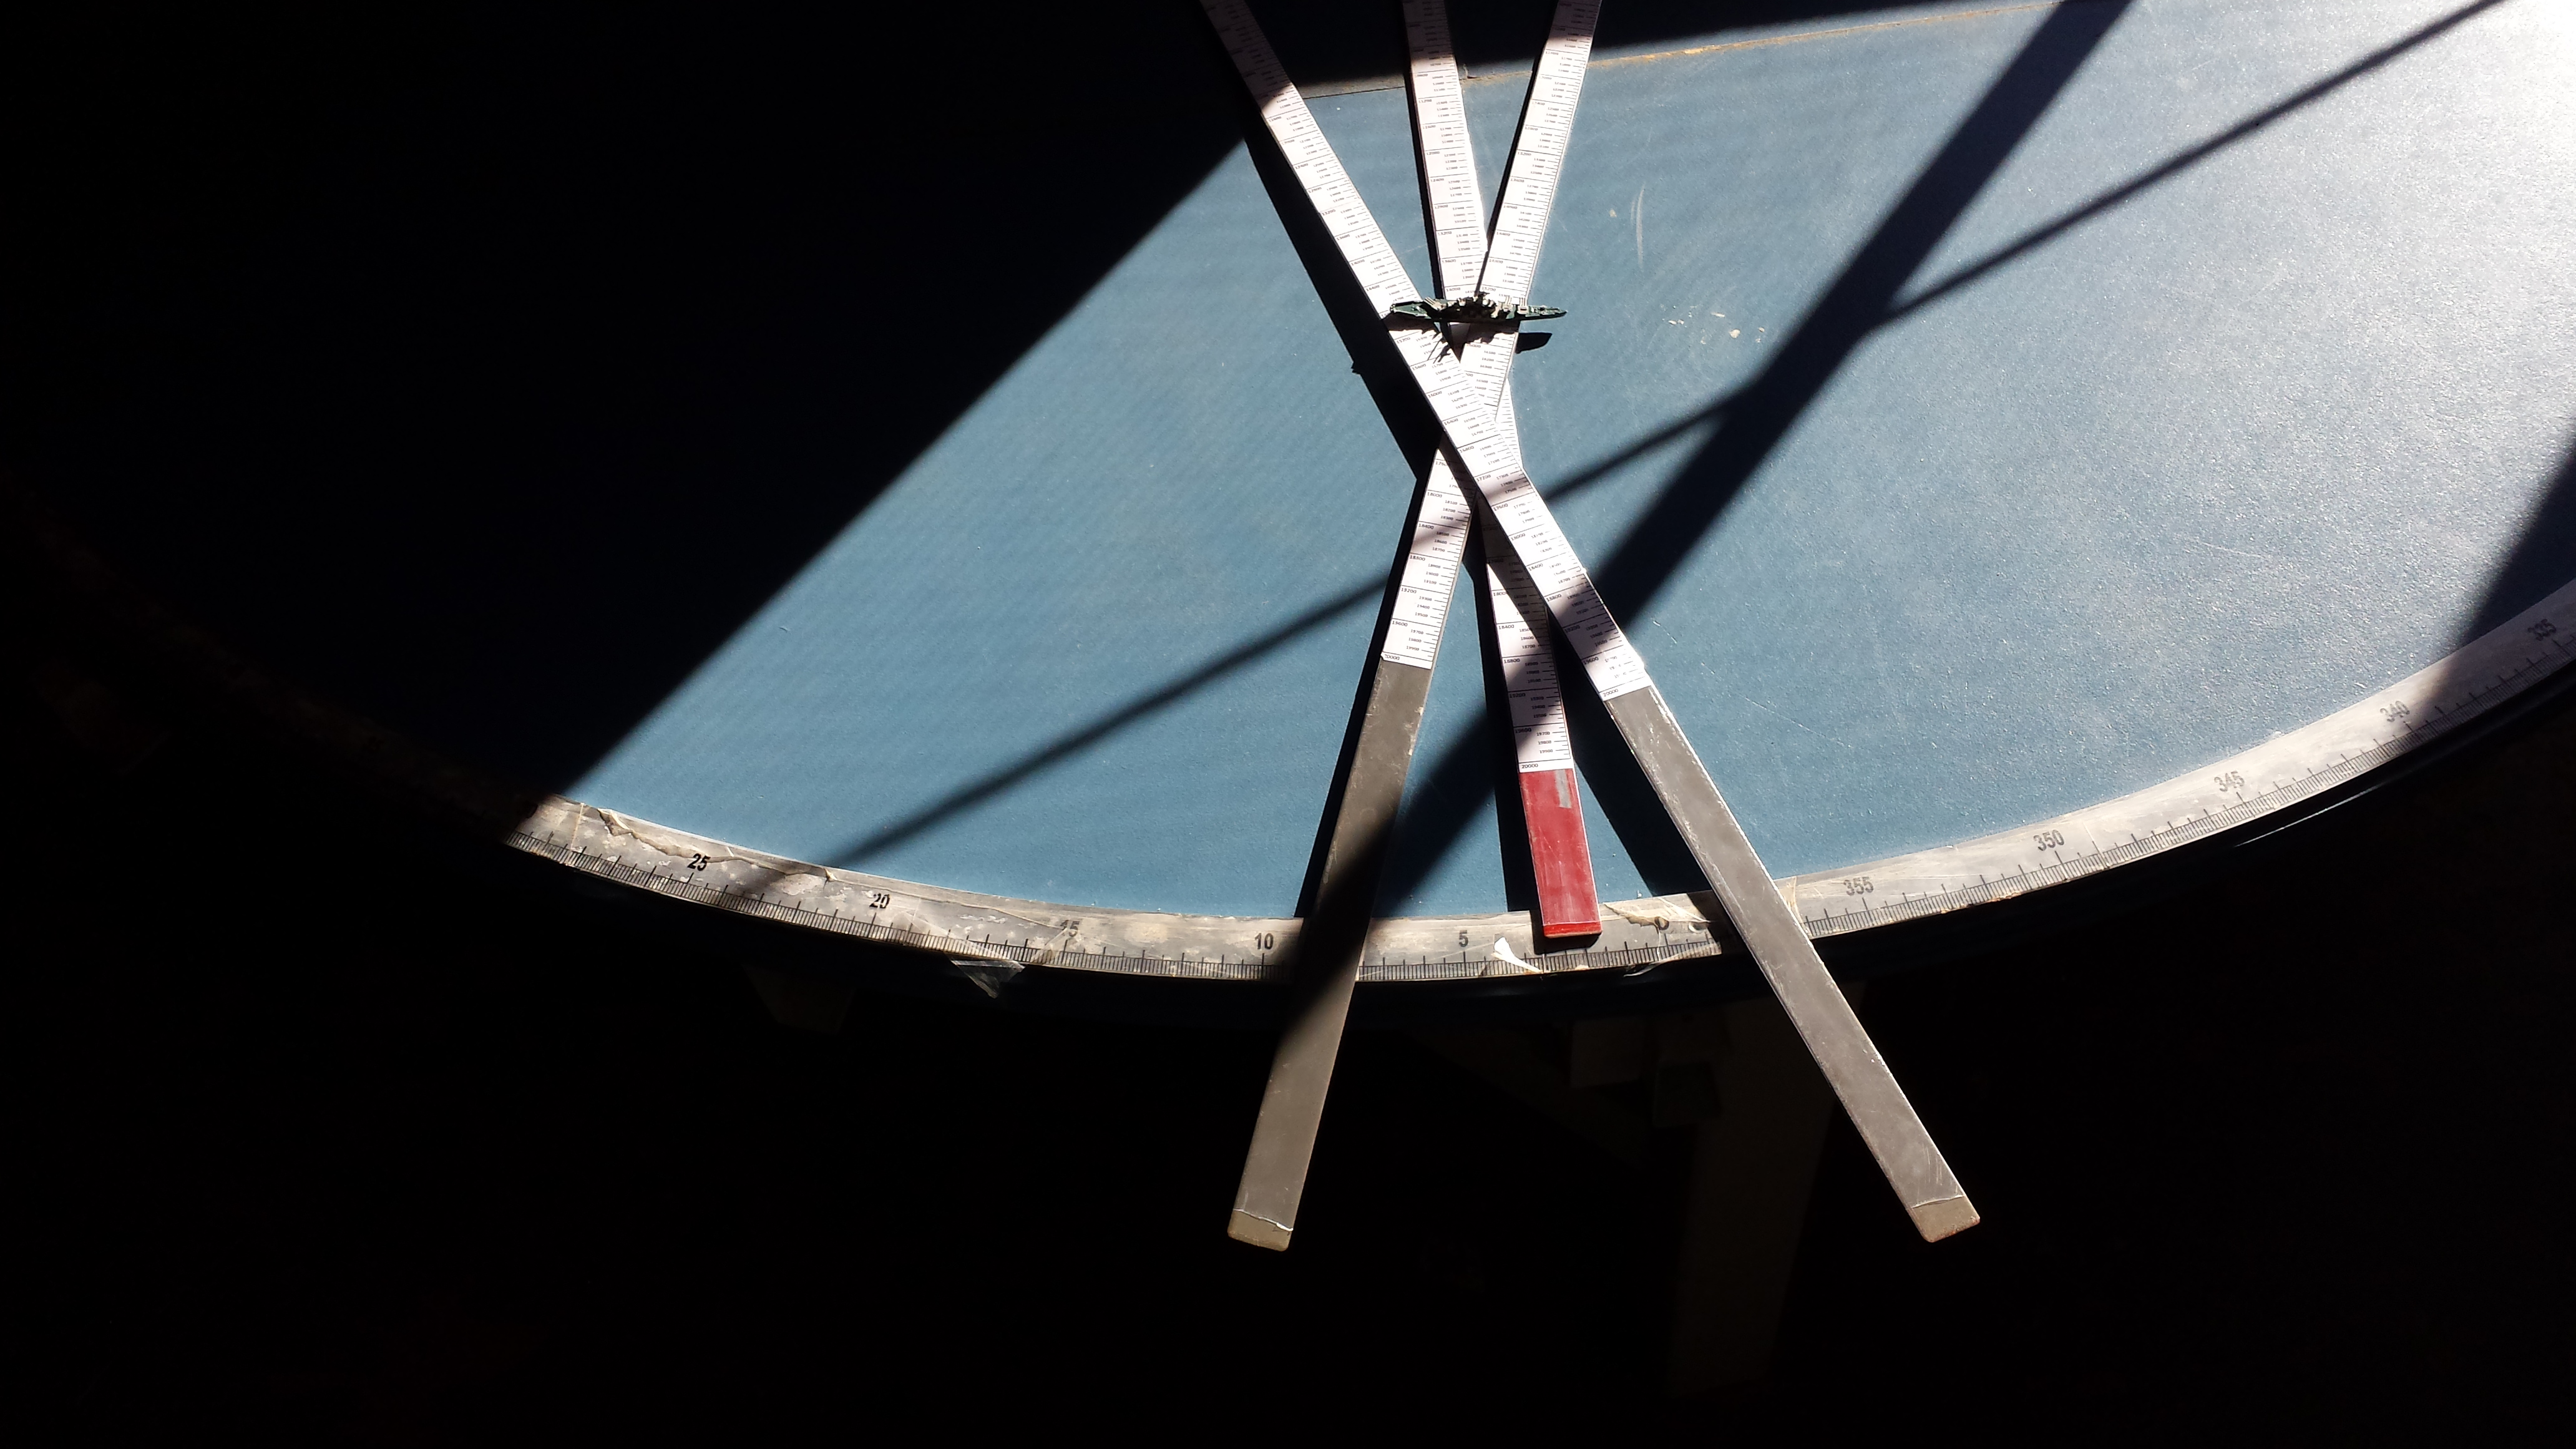
\includegraphics[width=0.5\textwidth]{test_image.jpg}
  \caption{I can embed images too}
\end{figure}

\noindent
We can make a table with centered elements:

\vspace{5mm}
\[ \left[ \begin{array}{c c c}
1.1754 & -0.8334 & 193.4191\\
0.2062 & 1.0380 & -141.0333\\
-0.0008 & 0.0007 & 1.0000\\
\end{array}
\right] \]
\vspace{5mm}

\noindent
There you go! That should be enough to get you started on LaTeX!

\end{document}
